\section{Experiments and results}\label{chapter4}

\subsection{Dataset}
We illustrate our neural network model on given datasets: training dataset, training labels and testing dataset.
Both training and testing datasets contain multiple samples with fixed-length of features.
We also observed that the original training dataset might be applied with PCA and reduced the dimension to $60000 \times 128$ matrix.
The training label is a $60000 \times 1$ matrix.
Similarly, the testing dataset is $10000 \times 128$ matrix.
Initially we split our dataset into $50,000$ training samples and $10,000$ test samples to find the number of iteration~\texttt{n\_iter} corresponding to the maximum cross-validation accuracy as our early stopping point.
Then we use all the $60,000$ samples to build our final neural network model.

\subsection{Experiment Setup}
We apply three layers neural network model with three different activation functions such as tanh, sigmoid and ReLu for the hidden layers as well as a Softmax activation function for the output layer.
We apply batch normalisation to the input for each layer to reduce the training time and make our model more resilient to parameter scale.
As for the regularisation techniques,
we use early stopping, drop out and weight decay to prevent over-fitting.
We use combinations of all the above setups to tune the hyperparameters for our neural network model,
in the end we successfully find the benchmark model to use for prediction with best accuracy and reasonable runtime.

\subsubsection{Multiprocessing speed up hyperparameters tuning}
We write a shell script to run all our tests in parallel in the virtual machines on the cloud,
this helps us fully utilise our computing resources to run multiple experiments with combinations of hyperparameters to tune our model.

\subsubsection{Hardware and software}
Figure~\ref{fig:hardware} shows the specification of the hardware we use for our experiments.
For the software, we are using python 3.6 to run the neural network model with a list of library dependencies specified in the requirements.txt file in our sample codes.

\begin{figure}
    \center{
        \includegraphics{resource/hardware.png}
    }
    \caption{Hardware to run the tests.}
    \label{fig:hardware}
\end{figure}


\subsubsection{Early stopping decides maximum number of iterations}
Early stopping is a form of regularisation technique we use to avoid over-fitting for our neutral network,
it guides us on how many iterations can be run before the model begins to over-fit.

In our experiment,
we observed that the benchmark model has an early-stopping at \texttt{n\_iter}=$44$.

\begin{figure}
	\centering{
	%\includegraphics[scale=.9]{Result_Multiplication_KL_Divergence_No_Noise_Comparison}
	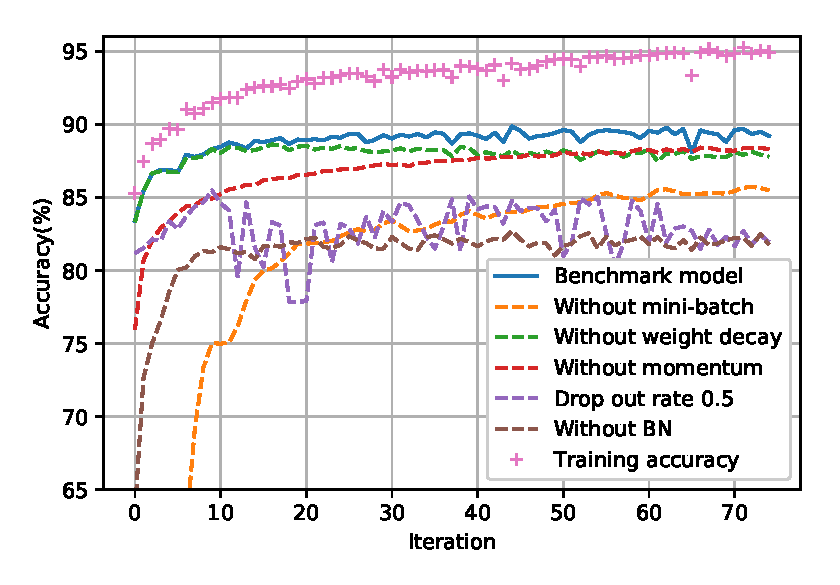
\includegraphics
    {resource/acc2.eps}}
    \caption{Results and parameters of different setups for 89.87}
    \label{fig:acc-iter}
\end{figure}

\subsection{Experiments Results}
\subsubsection{Optimal hyperparameters}

Table~\ref{table:best-four-steps} shows results and hyperparameters with optimal and sub-optimal coefficients. The benchmark model achieved the accuracy of $89.9\%$.

\begin{table}
\caption{Results and parameters of the best four setups.}
\label{table:best-four-steps}
{\footnotesize
% \label{tab:ci}\begin{tabular}{l|lll}
%  \hline
% \texttt{ORL} dataset & \textsc{rre} & \textsc{acc} & \textsc{nmi}\tabularnewline
%  \hline
% \textsc{nmf} no noise & 0.1583 (0.1581, 0.1584) & 0.7364 (0.731, 0.742) & 0.8536 (0.8506, 0.8567)\tabularnewline
% \hline
% \end{tabular}}
\centering
\begin{tabular}{@{}llllll@{}}
\toprule
Experiment                & Test 1  & Test 2           & Test 3           & Test 4  & Test 5  \\ \midrule
Runtime(mins)             & 2.3     & 2.7              & 3.6              & 17.2    & 10.8    \\
Accurarcy                 & 89.9\%  & 89.7\%           & 89.8\%           & 90.0\%  & 89.3\%  \\
Initialisation            & Xavier  & Uniform$(-1,1)$ & Uniform$(-1,1)$ & Xavier  & Xavier  \\
Batch size                & 1500    & 1500             & 1500             & 1500    & 1500    \\
Hidden layer nodes        & 160     & 150              & 150              & 900     & 160     \\
Activation function       & $\tanh$ & $\tanh$          & $\tanh$          & $\tanh$ & sigmoid \\
Weight decay rate         & 0.0007  & 0.0007           & 0.0007           & 0.007   & 0.007   \\
Momentum rate             & 0.9     & 0.9              & 0.92             & 0.9     & 0.9     \\
Dropout rate              & 0.95    & 1.0              & 1.0              & 0.5     & 0.95    \\
Learning rate             & 0.11    & 0.05             & 0.05             & 0.11    & 0.11    \\
Early stopping iterations & 44      & 54               & 66               & 158     & 282     \\ \bottomrule
\end{tabular}
%\csvautobooktabular{resource/table1.csv}
}
\end{table}

\begin{table}
\caption{Results and parameters of different setups for 89.87 results.}
{\footnotesize \centering
\begin{tabular}{@{}lrrrrr@{}}
\toprule
Experiment                & Test 1  & Drop out 50\% & Weight decay & Momentum & Mini-Batch \\ \midrule
Runtime(minutes)          & 2.3     & 0.5        & 8.6          & 0.8      & 7.6           \\
Accurarcy                 & 89.9\%  & 85.5\%     & 89.4\%       & 88.6\%   & 87.5\%        \\
Initialisation            & Xavier  & Xavier     & Xavier       & Xavier   & Xavier        \\
Batch size                & 1500    & 1500       & 1500         & 1500     & 60000         \\
Hidden layer nodes        & 160     & 160        & 160          & 160      & 160           \\
Activation function       & $\tanh$ & $\tanh$    & $\tanh$      & $\tanh$  & $\tanh$       \\
Weight decay rate         & 0.0007  & 0.0007     & 0.0007       & 0        & 0.007         \\
Momentum rate             & 0.9     & 0.9        & 0            & 0.9      & 0.9           \\
Dropout rate              & 0.95    & 0.5        & 0.95         & 0.95     & 0.95          \\
Learning rate             & 0.11    & 0.11       & 0.11         & 0.11     & 0.11          \\
Early stopping iterations & 44      & 9          & 198          & 16       & 177           \\ \bottomrule
\end{tabular}
}
\end{table}

% \begin{figure}
%     \center{\includegraphics
%     {resource/acc.eps}}
%     \caption{\label{fig:my-label2}Results and parameters of different setups for 89.87 results.}
% \end{figure}

\begin{figure}
    \center{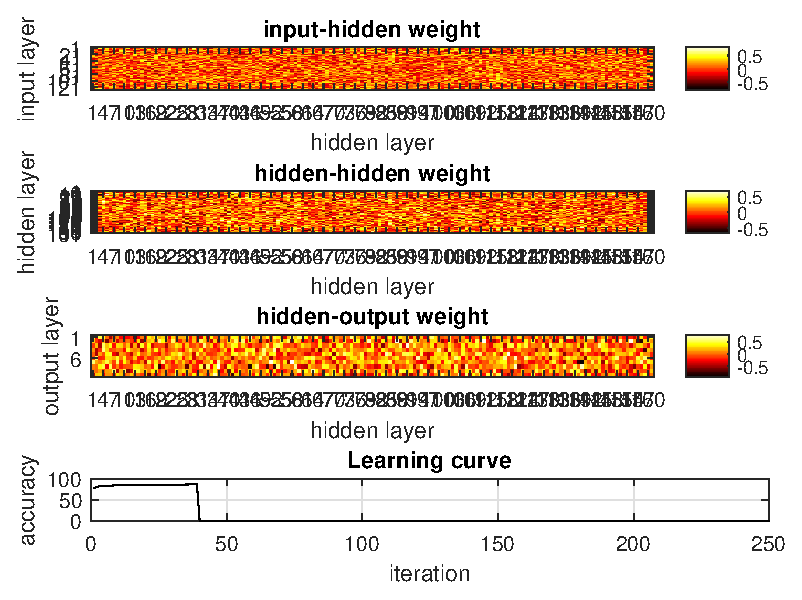
\includegraphics
    {resource/figure2.eps}}
    \caption{\label{fig:my-label3}Weight Matrix on multiple layers.}
\end{figure}


\subsection{Experiments Results}

\subsubsection{Vectorisation dramatically improves the speed of training}
We used vectorisation from numpy to perform fast computation and transformation of the data rather than using the traditional for-loop,
these operations includes matrix concatenation, multiplication, divide using Numpy libraries.

\subsubsection{Batch normalisation significantly improves the accuracy}


\subsubsection{Weight decaying prevents over-fitting}


\subsubsection{dropout does not help here}
